\chapter{Anexos: Capturas del Simulador}
\label{sec.anexo:capturas}

Se presentan a continuación las capturas de pantalla obtenidas en el simulador virtual del Aula Moisan para cada una de las condiciones de ensayo analizadas.

\section{Capturas de Ensayos de Vacío y Carga con Factor de Potencia Unitario}

\begin{figure}[!ht]
    \centering
    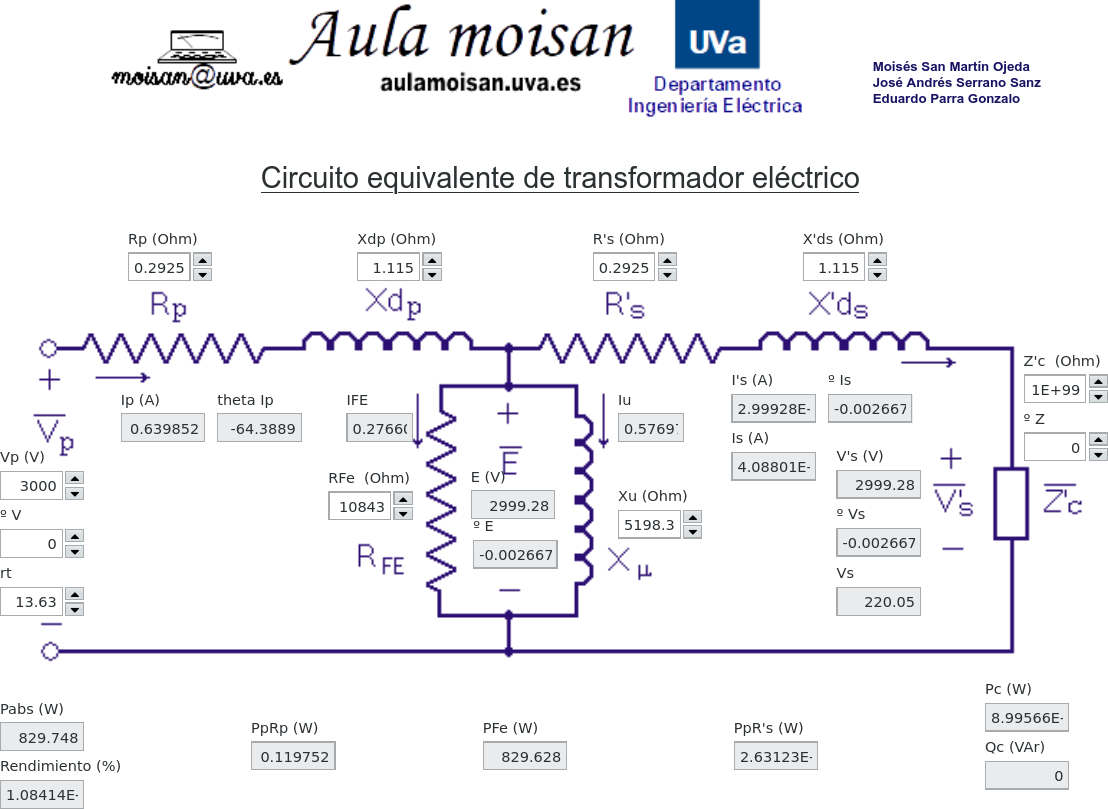
\includegraphics[width=0.7\textwidth]{images/fig_vacio.png}
    \caption{Ensayo de vacío ($Z'_c = \infty$).}
    \label{fig.anexo:vacio}
\end{figure}

\begin{figure}[!ht]
    \centering
    \begin{subfigure}[t]{0.48\textwidth}
        \centering
        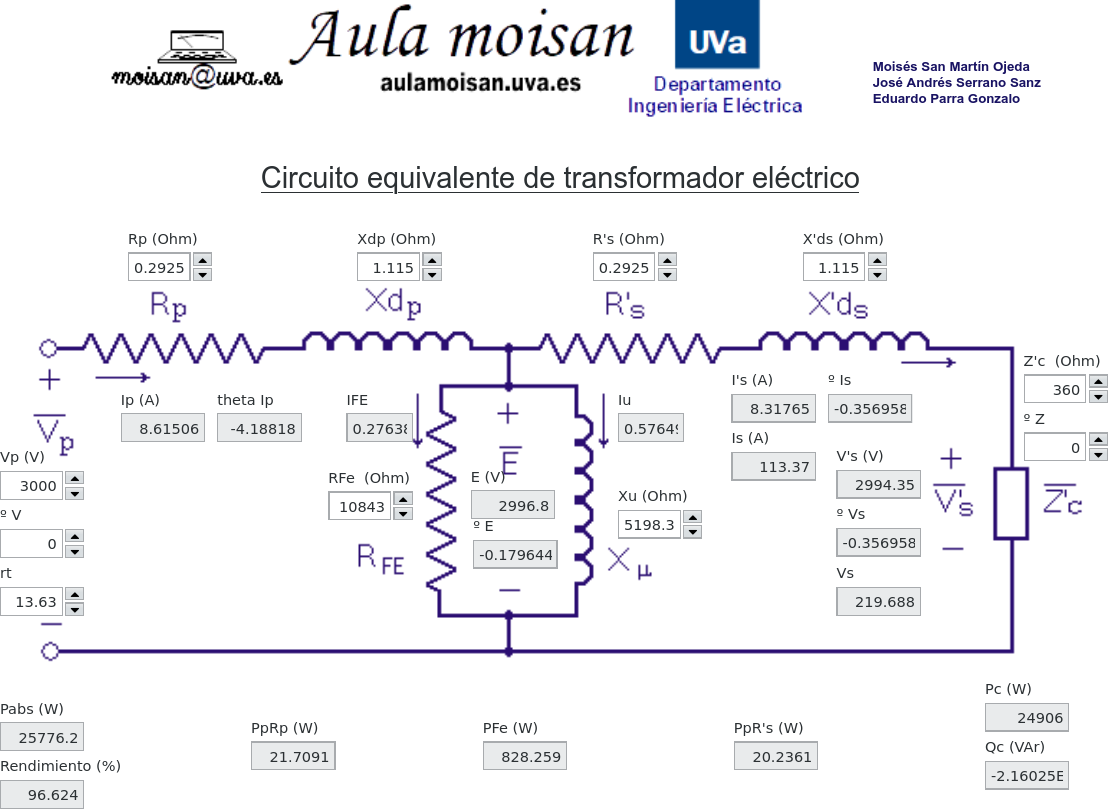
\includegraphics[width=\textwidth]{images/fig_carga_25_fp1.png}
        \caption{Carga al $\SI{25}{\percent}$ ($Z'_c = \SI{360}{\ohm}$).}
        \label{fig.anexo:carga_25}
    \end{subfigure}
    \hfill
    \begin{subfigure}[t]{0.48\textwidth}
        \centering
        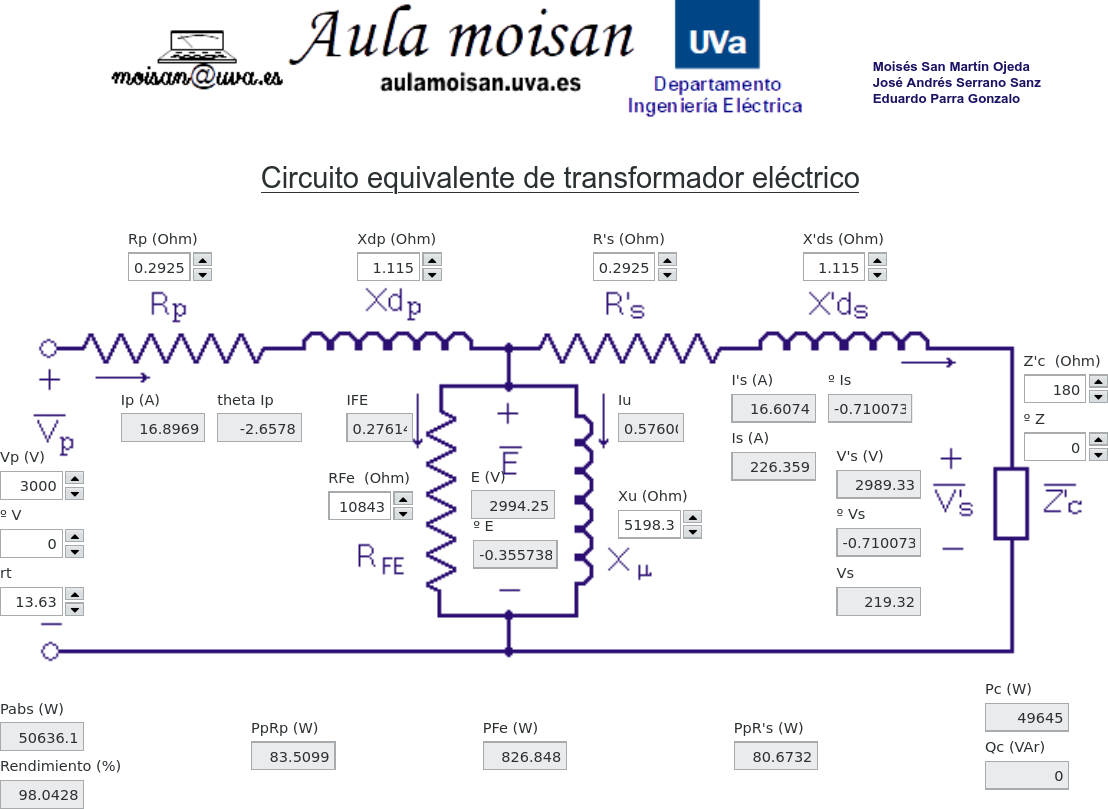
\includegraphics[width=\textwidth]{images/fig_carga_50_fp1.png}
        \caption{Carga al $\SI{50}{\percent}$ ($Z'_c = \SI{180}{\ohm}$).}
        \label{fig.anexo:carga_50}
    \end{subfigure}
    \vskip\baselineskip
    \begin{subfigure}[t]{0.48\textwidth}
        \centering
        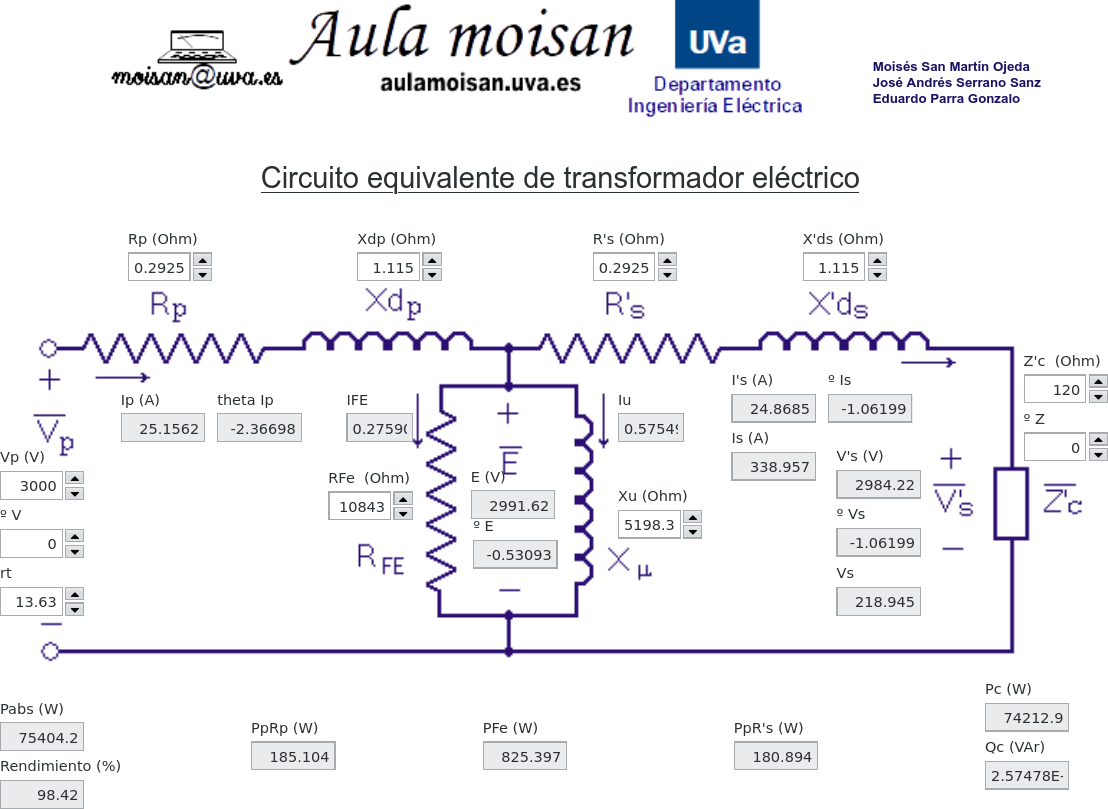
\includegraphics[width=\textwidth]{images/fig_carga_75_fp1.png}
        \caption{Carga al $\SI{75}{\percent}$ ($Z'_c = \SI{120}{\ohm}$).}
        \label{fig.anexo:carga_75}
    \end{subfigure}
    \hfill
    \begin{subfigure}[t]{0.48\textwidth}
        \centering
        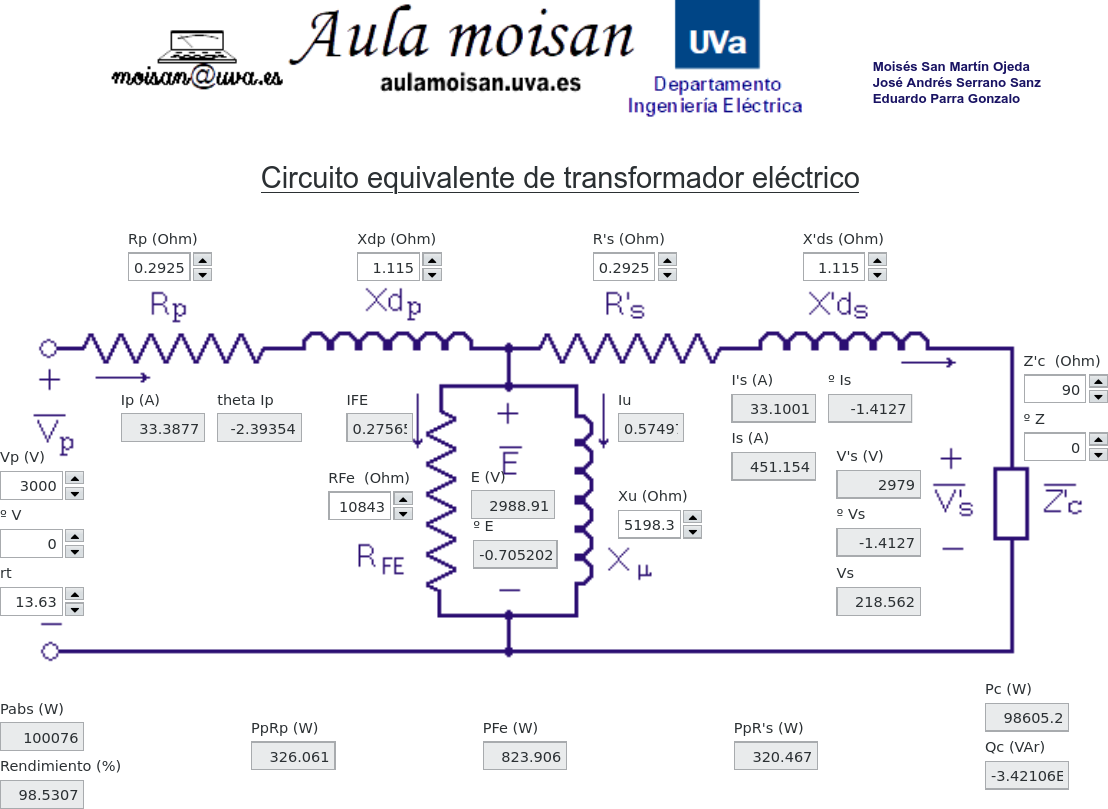
\includegraphics[width=\textwidth]{images/fig_carga_100_fp1.png}
        \caption{Carga al $\SI{100}{\percent}$ ($Z'_c = \SI{90}{\ohm}$).}
        \label{fig.anexo:carga_100}
    \end{subfigure}
    \caption{Simulaciones de carga resistiva ($f_p = 1,0$).}
    \label{fig.anexo:grupo_carga_resistiva}
\end{figure}

\newpage

\section{Capturas de Ensayos de Carga con Factor de Potencia Inductivo}

\begin{figure}[!ht]
    \centering
    \begin{subfigure}[t]{0.48\textwidth}
        \centering
        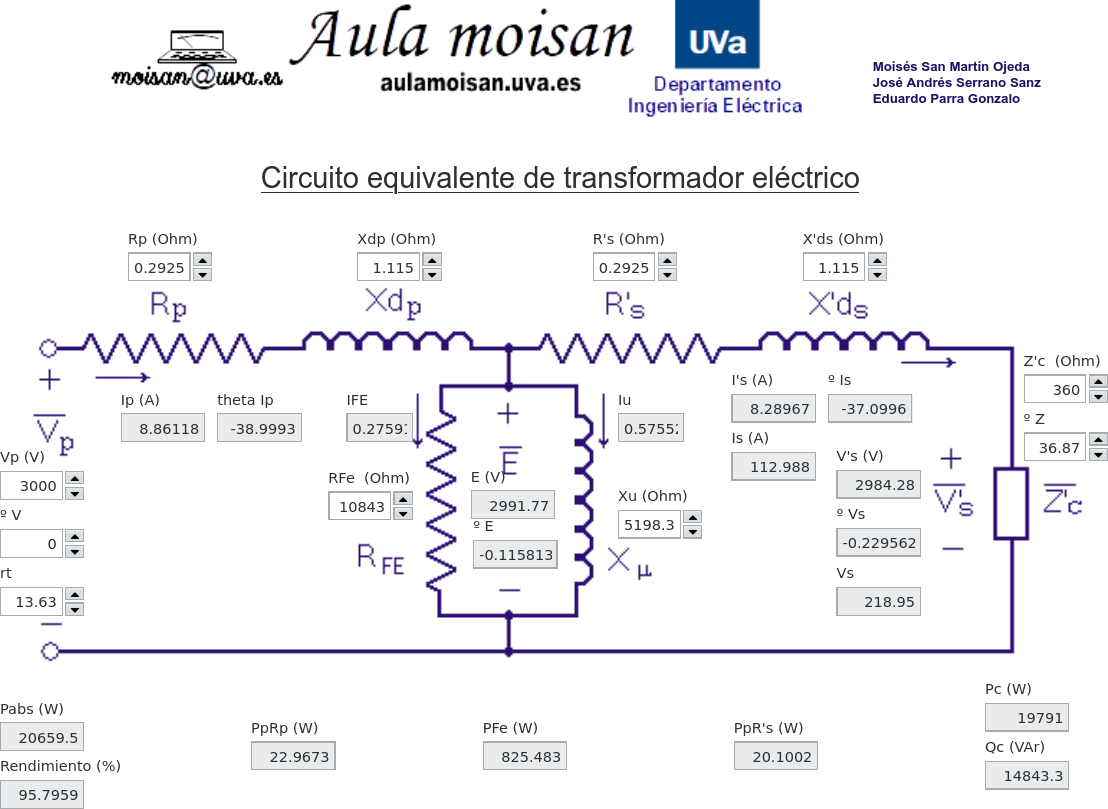
\includegraphics[width=\textwidth]{images/fig_carga_25_fp08ind.png}
        \caption{Carga al $\SI{25}{\percent}$ ($Z'_c = \SI{360}{\ohm}$).}
        \label{fig.anexo:carga_25_ind}
    \end{subfigure}
    \hfill
    \begin{subfigure}[t]{0.48\textwidth}
        \centering
        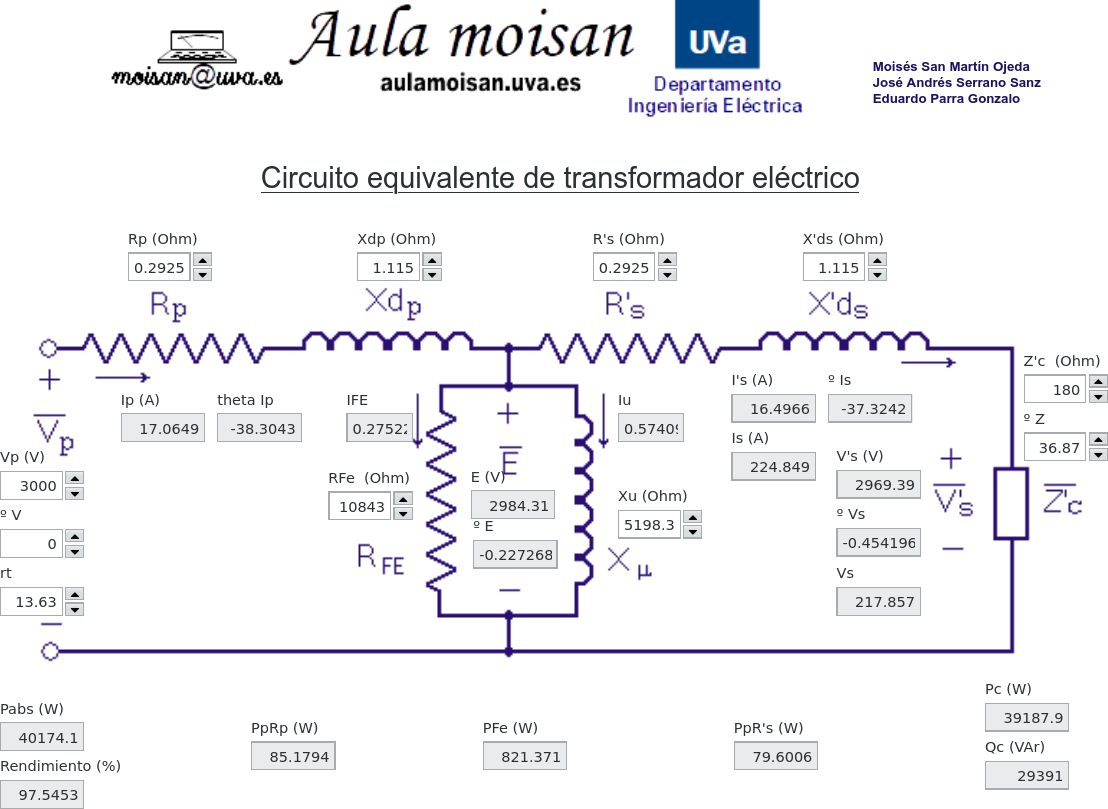
\includegraphics[width=\textwidth]{images/fig_carga_50_fp08ind.png}
        \caption{Carga al $\SI{50}{\percent}$ ($Z'_c = \SI{180}{\ohm}$).}
        \label{fig.anexo:carga_50_ind}
    \end{subfigure}
    \vskip\baselineskip
    \begin{subfigure}[t]{0.48\textwidth}
        \centering
        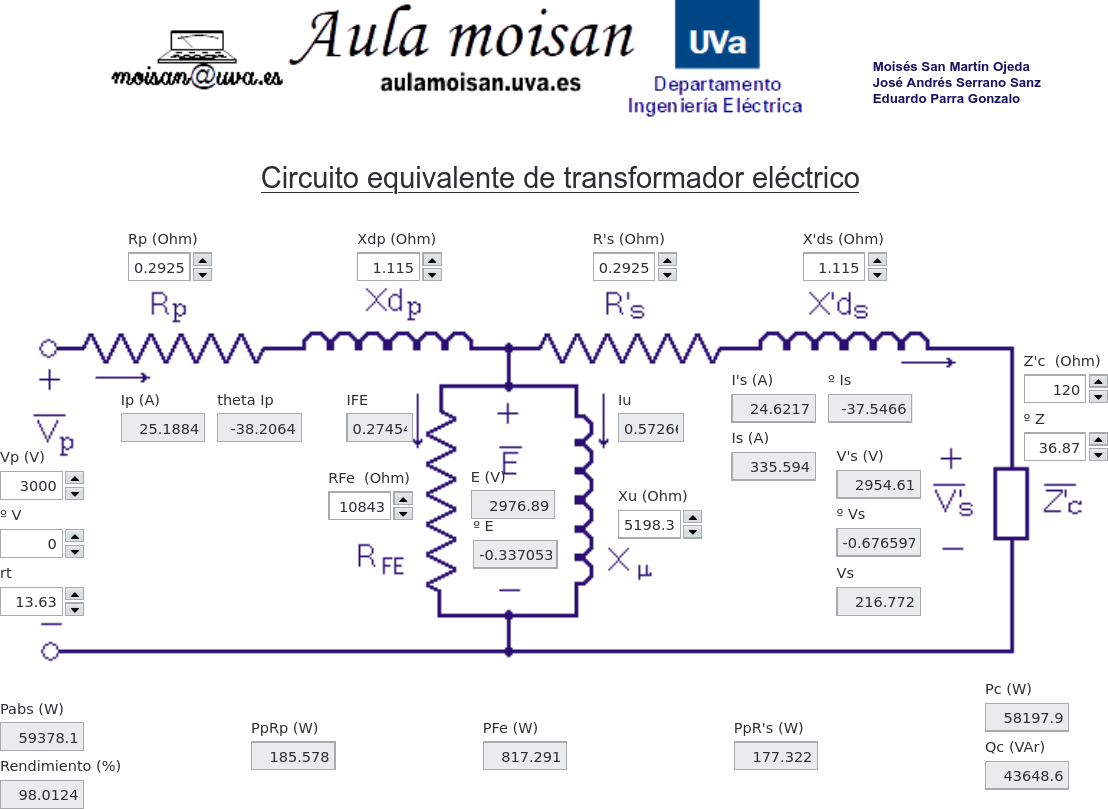
\includegraphics[width=\textwidth]{images/fig_carga_75_fp08ind.png}
        \caption{Carga al $\SI{75}{\percent}$ ($Z'_c = \SI{120}{\ohm}$).}
        \label{fig.anexo:carga_75_ind}
    \end{subfigure}
    \hfill
    \begin{subfigure}[t]{0.48\textwidth}
        \centering
        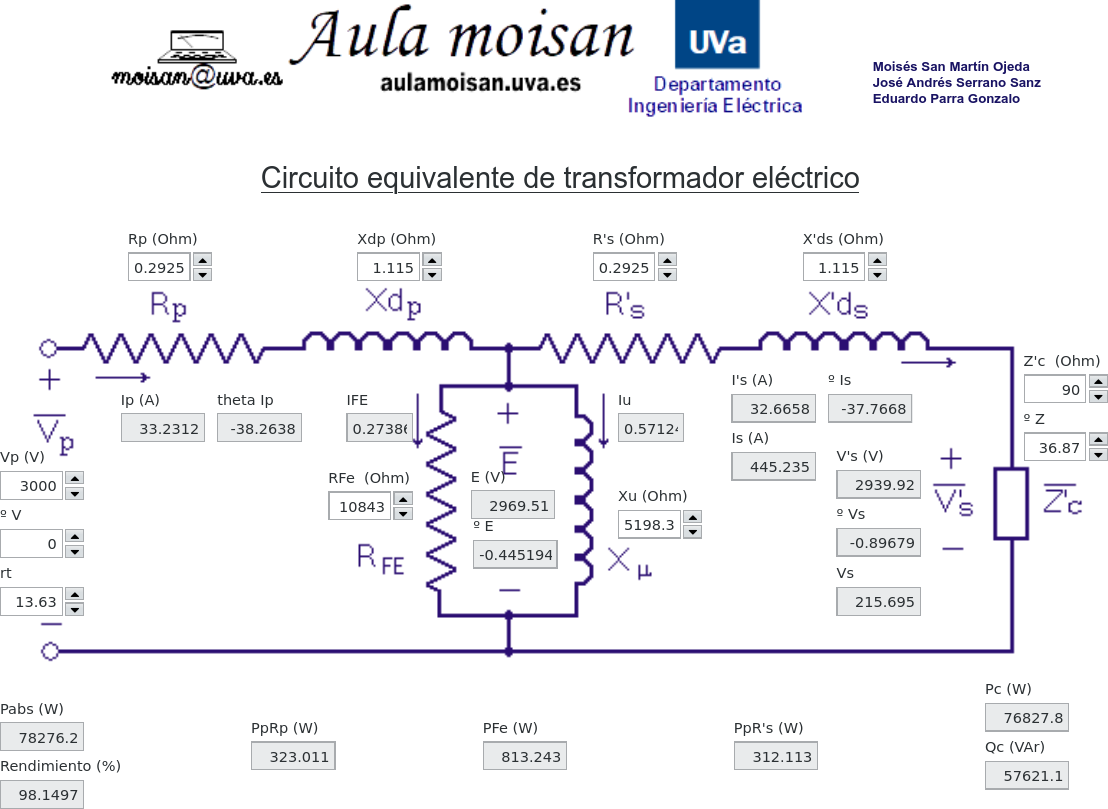
\includegraphics[width=\textwidth]{images/fig_carga_100_fp08ind.png}
        \caption{Carga al $\SI{100}{\percent}$ ($Z'_c = \SI{90}{\ohm}$).}
        \label{fig.anexo:carga_100_ind}
    \end{subfigure}
    \caption{Simulaciones de carga inductiva ($f_p = 0,8$ ind, $\theta_Z = +36,87^\circ$).}
    \label{fig.anexo:grupo_carga_inductiva}
\end{figure}

\newpage

\section{Capturas de Ensayos de Carga con Factor de Potencia Capacitivo}

\begin{figure}[!ht]
    \centering
    \begin{subfigure}[t]{0.48\textwidth}
        \centering
        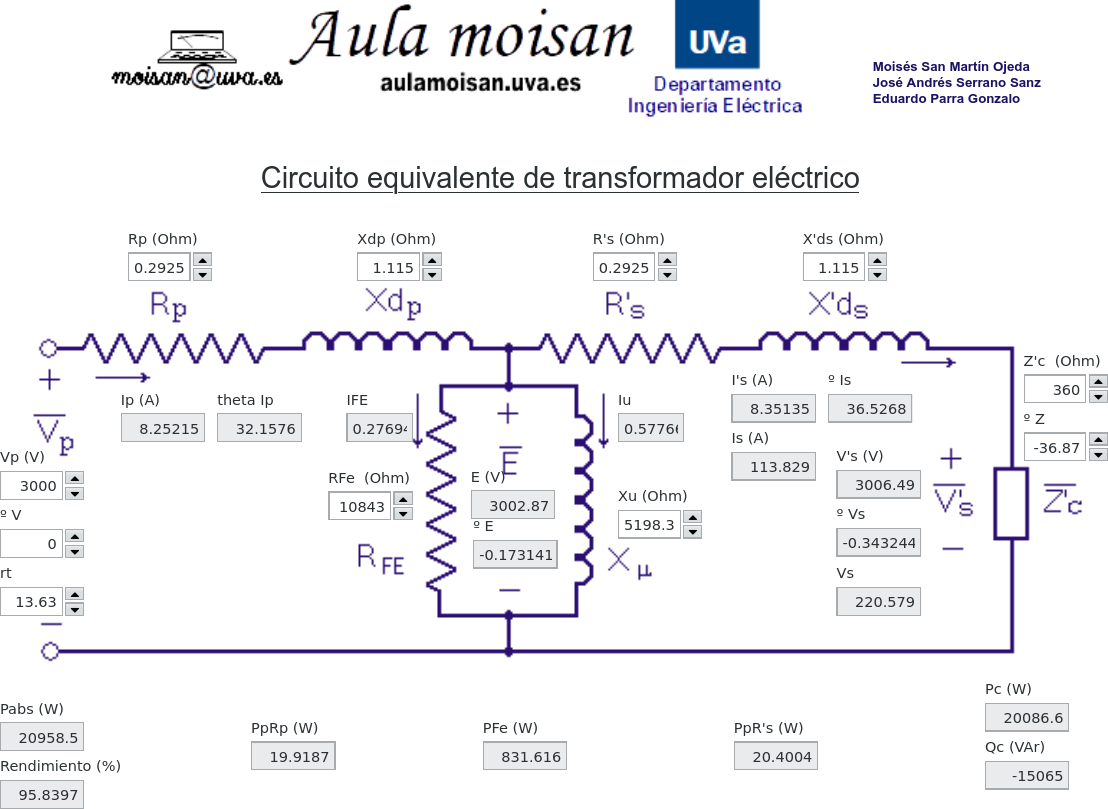
\includegraphics[width=\textwidth]{images/fig_carga_25_fp08cap.png}
        \caption{Carga al $\SI{25}{\percent}$ ($Z'_c = \SI{360}{\ohm}$).}
        \label{fig.anexo:carga_25_cap}
    \end{subfigure}
    \hfill
    \begin{subfigure}[t]{0.48\textwidth}
        \centering
        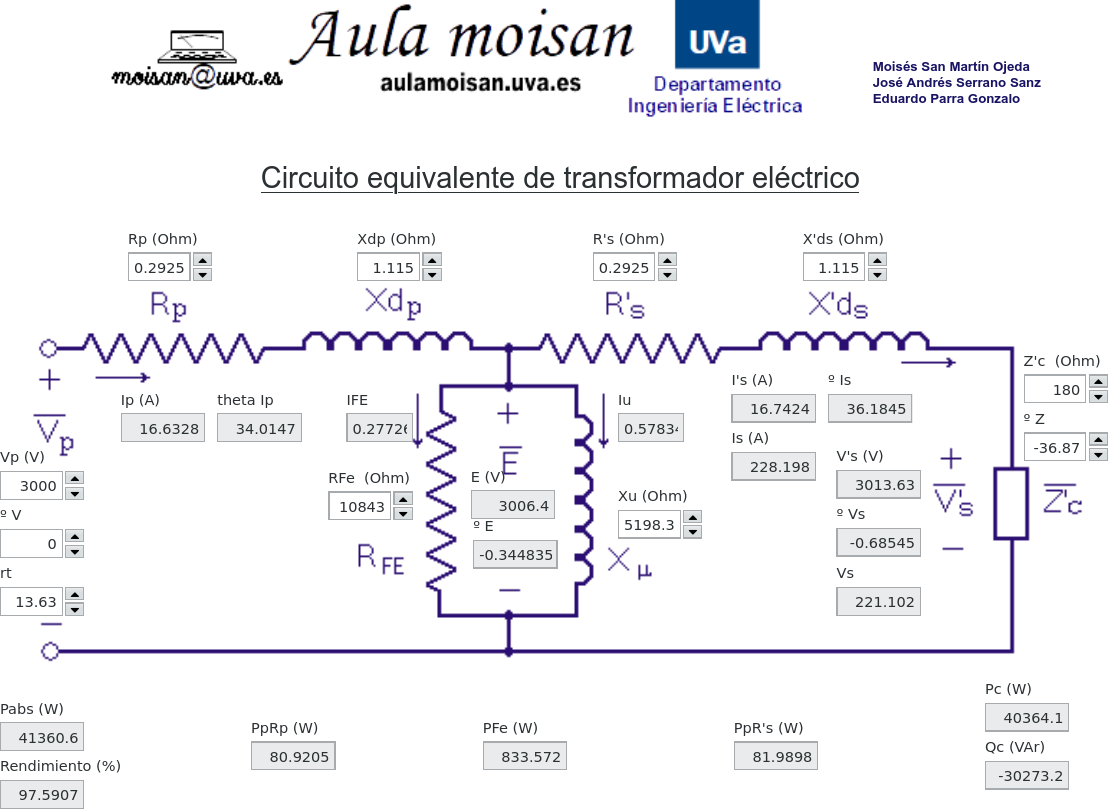
\includegraphics[width=\textwidth]{images/fig_carga_50_fp08cap.png}
        \caption{Carga al $\SI{50}{\percent}$ ($Z'_c = \SI{180}{\ohm}$).}
        \label{fig.anexo:carga_50_cap}
    \end{subfigure}
    \vskip\baselineskip
    \begin{subfigure}[t]{0.48\textwidth}
        \centering
        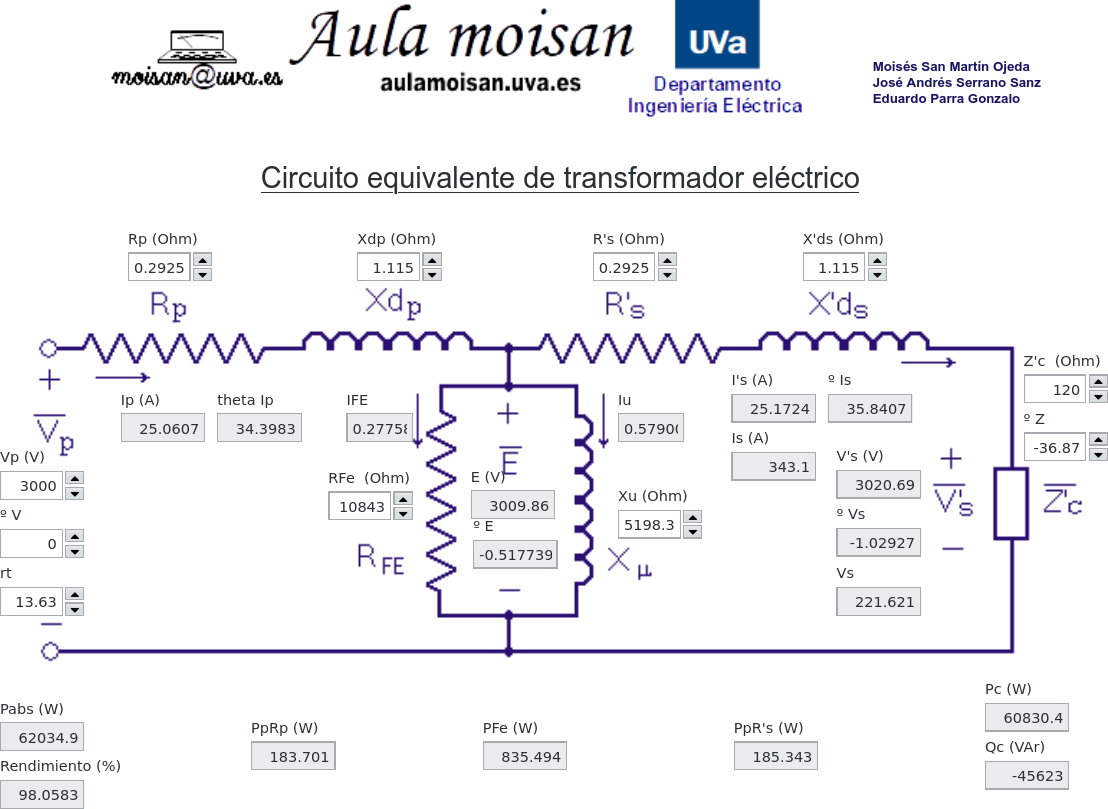
\includegraphics[width=\textwidth]{images/fig_carga_75_fp08cap.png}
        \caption{Carga al $\SI{75}{\percent}$ ($Z'_c = \SI{120}{\ohm}$).}
        \label{fig.anexo:carga_75_cap}
    \end{subfigure}
    \hfill
    \begin{subfigure}[t]{0.48\textwidth}
        \centering
        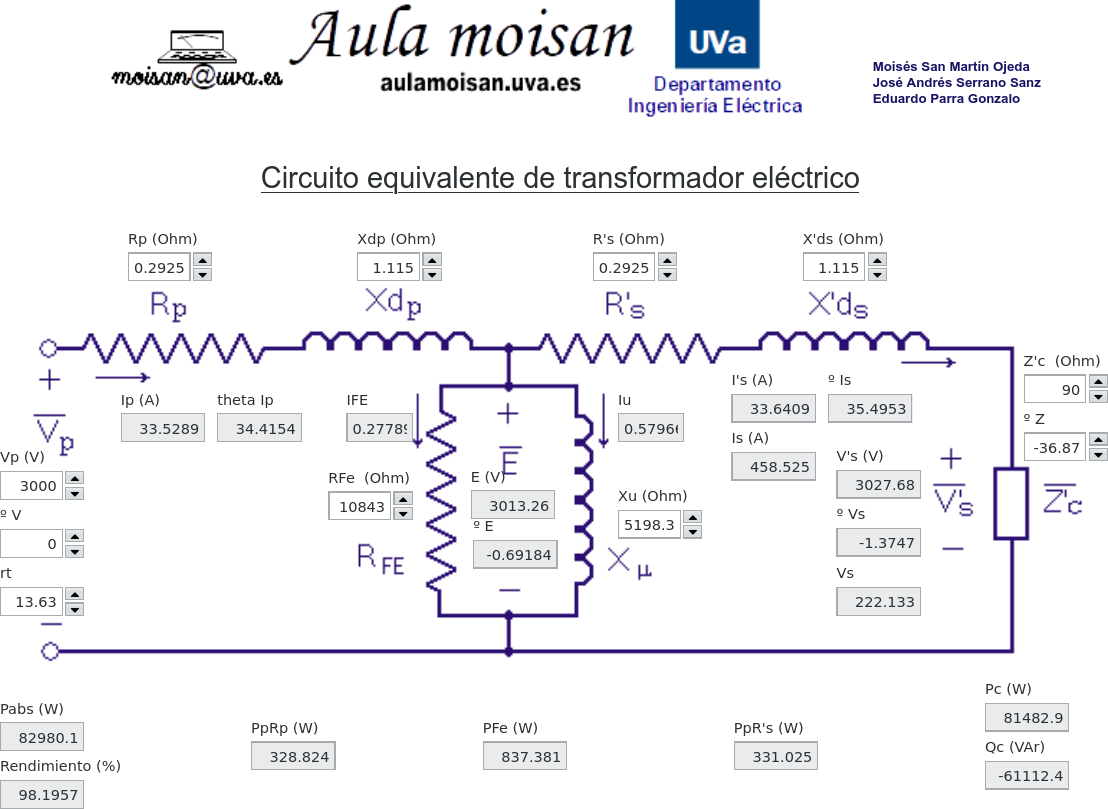
\includegraphics[width=\textwidth]{images/fig_carga_100_fp08cap.png}
        \caption{Carga al $\SI{100}{\percent}$ ($Z'_c = \SI{90}{\ohm}$).}
        \label{fig.anexo:carga_100_cap}
    \end{subfigure}
    \caption{Simulaciones de carga capacitiva ($f_p = 0,8$ cap, $\theta_Z = -36,87^\circ$).}
    \label{fig.anexo:grupo_carga_capacitiva}
\end{figure}

\newpage

\section{Capturas de Ensayos de Cortocircuito}

\begin{figure}[!ht]
    \centering
    \begin{subfigure}[t]{0.48\textwidth}
        \centering
        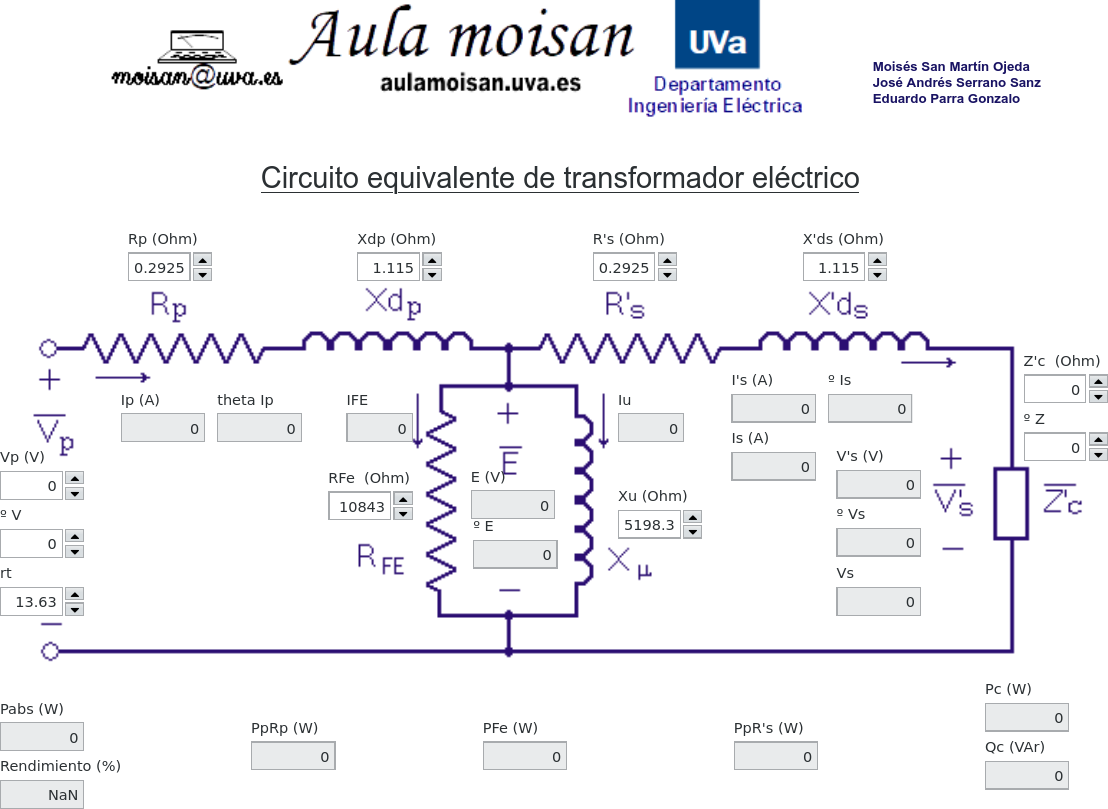
\includegraphics[width=\textwidth]{images/fig_cc_controlado_0V.png}
        \caption{$V_p = \SI{0}{\volt}$.}
        \label{fig.anexo:cc_0V}
    \end{subfigure}
    \hfill
    \begin{subfigure}[t]{0.48\textwidth}
        \centering
        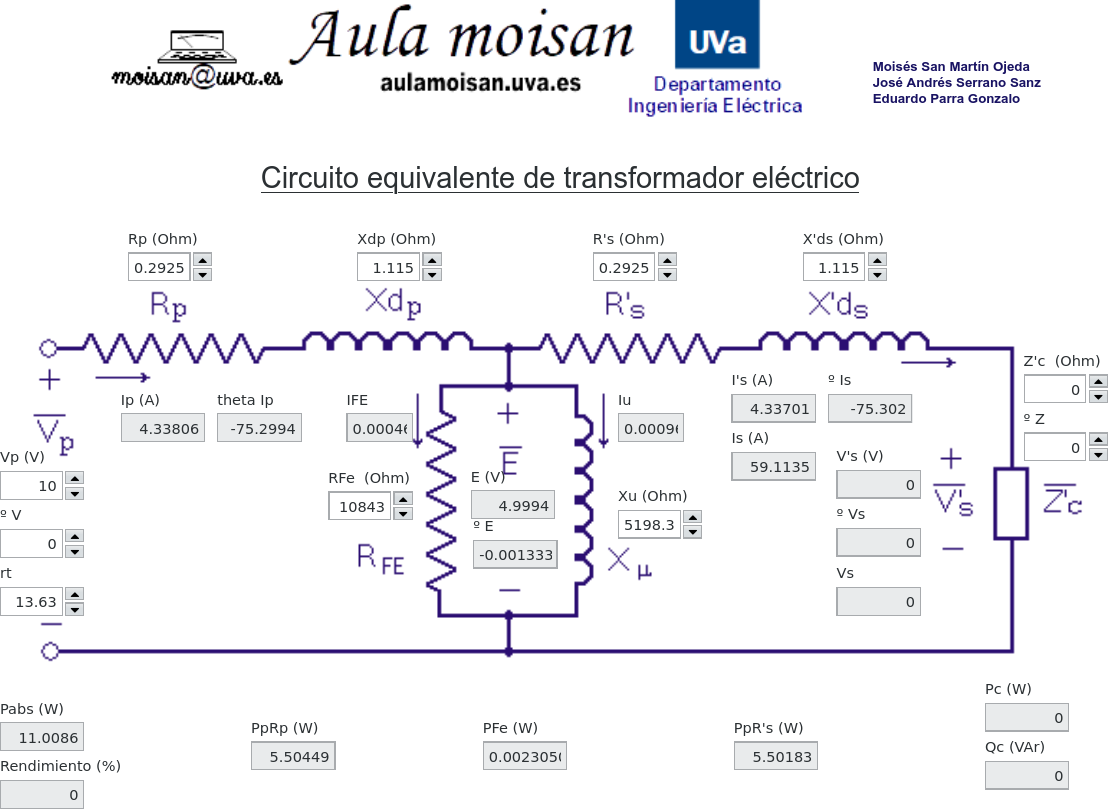
\includegraphics[width=\textwidth]{images/fig_cc_controlado_10V.png}
        \caption{$V_p = \SI{10}{\volt}$.}
        \label{fig.anexo:cc_10V}
    \end{subfigure}
    \vskip\baselineskip
    \begin{subfigure}[t]{0.48\textwidth}
        \centering
        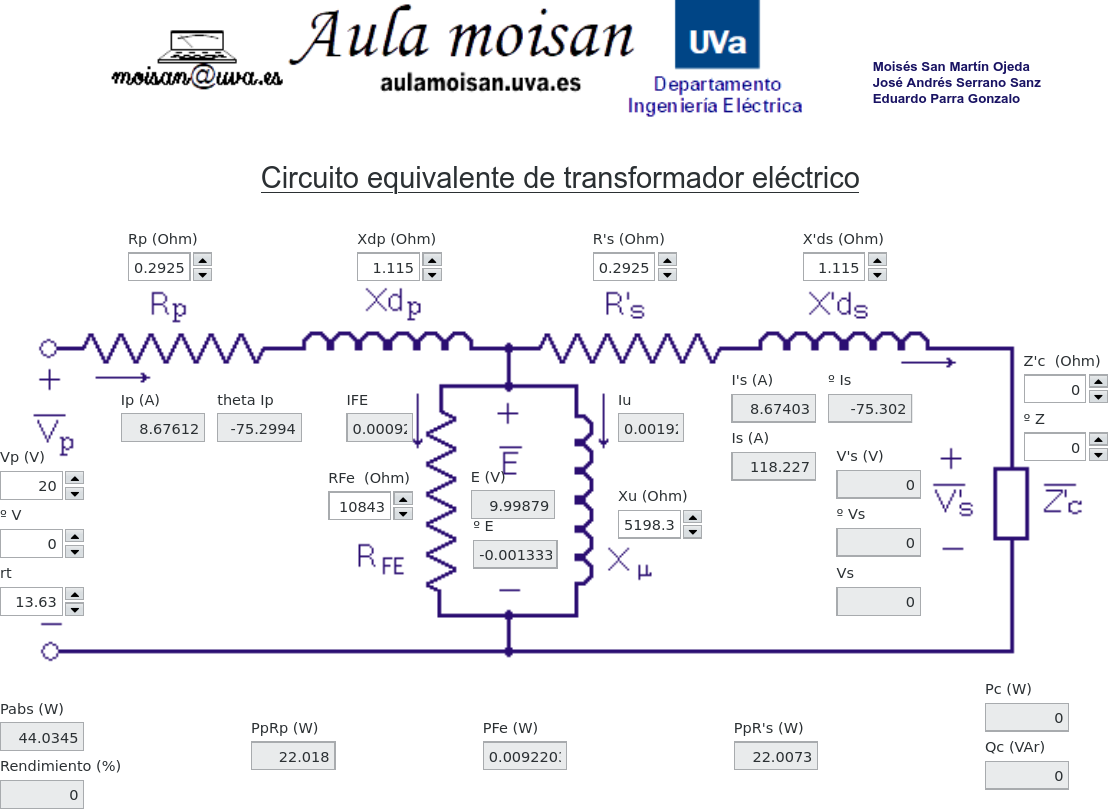
\includegraphics[width=\textwidth]{images/fig_cc_controlado_20V.png}
        \caption{$V_p = \SI{20}{\volt}$.}
        \label{fig.anexo:cc_20V}
    \end{subfigure}
    \hfill
    \begin{subfigure}[t]{0.48\textwidth}
        \centering
        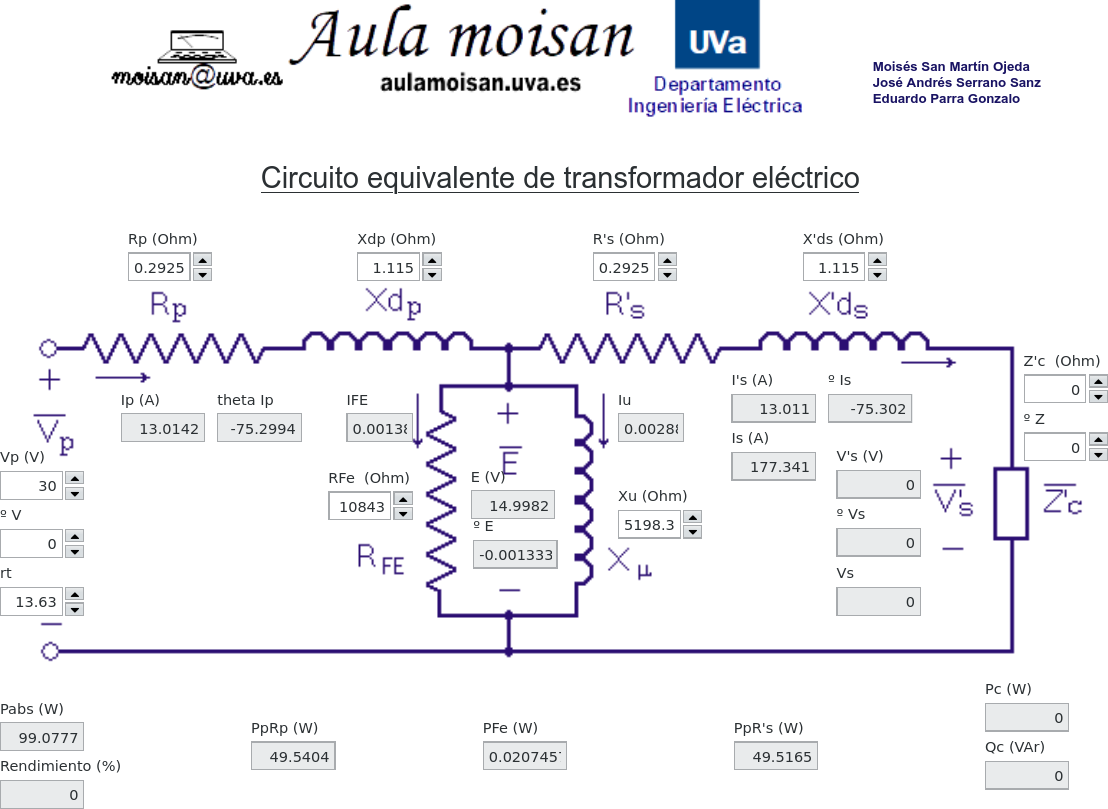
\includegraphics[width=\textwidth]{images/fig_cc_controlado_30V.png}
        \caption{$V_p = \SI{30}{\volt}$.}
        \label{fig.anexo:cc_30V}
    \end{subfigure}
    \vskip\baselineskip
    \begin{subfigure}[t]{0.48\textwidth}
        \centering
        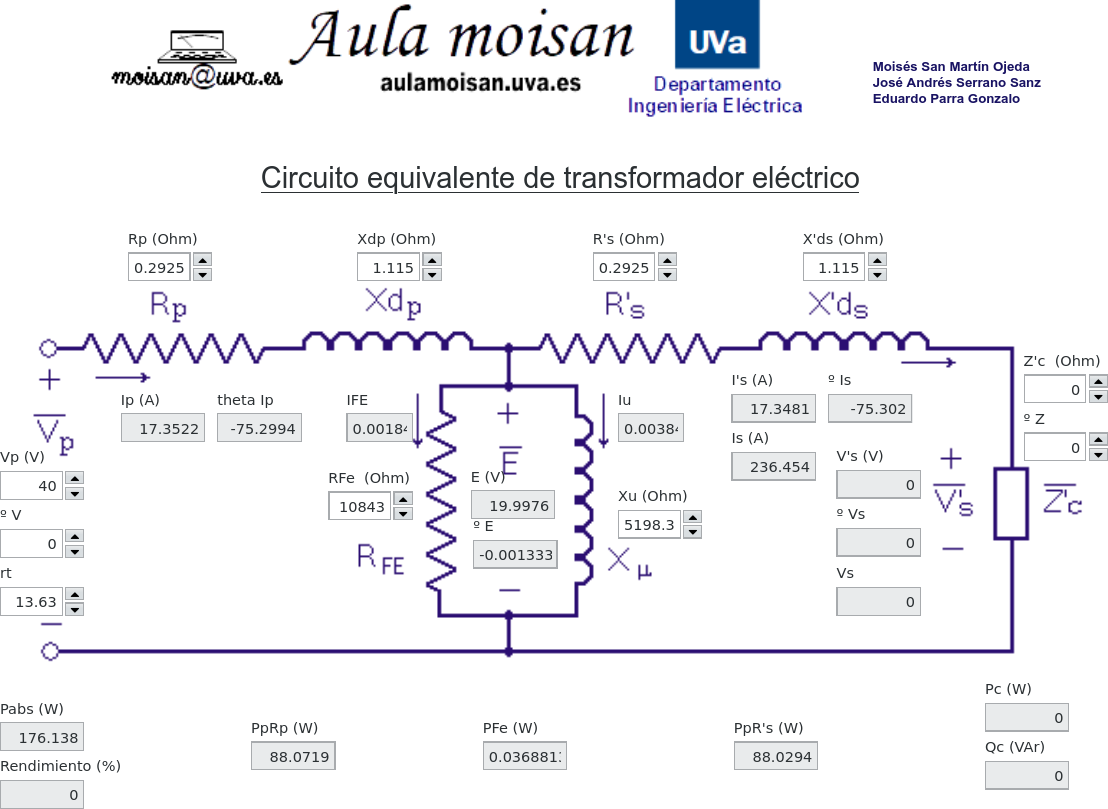
\includegraphics[width=\textwidth]{images/fig_cc_controlado_40V.png}
        \caption{$V_p = \SI{40}{\volt}$.}
        \label{fig.anexo:cc_40V}
    \end{subfigure}
    \hfill
    \begin{subfigure}[t]{0.48\textwidth}
        \centering
        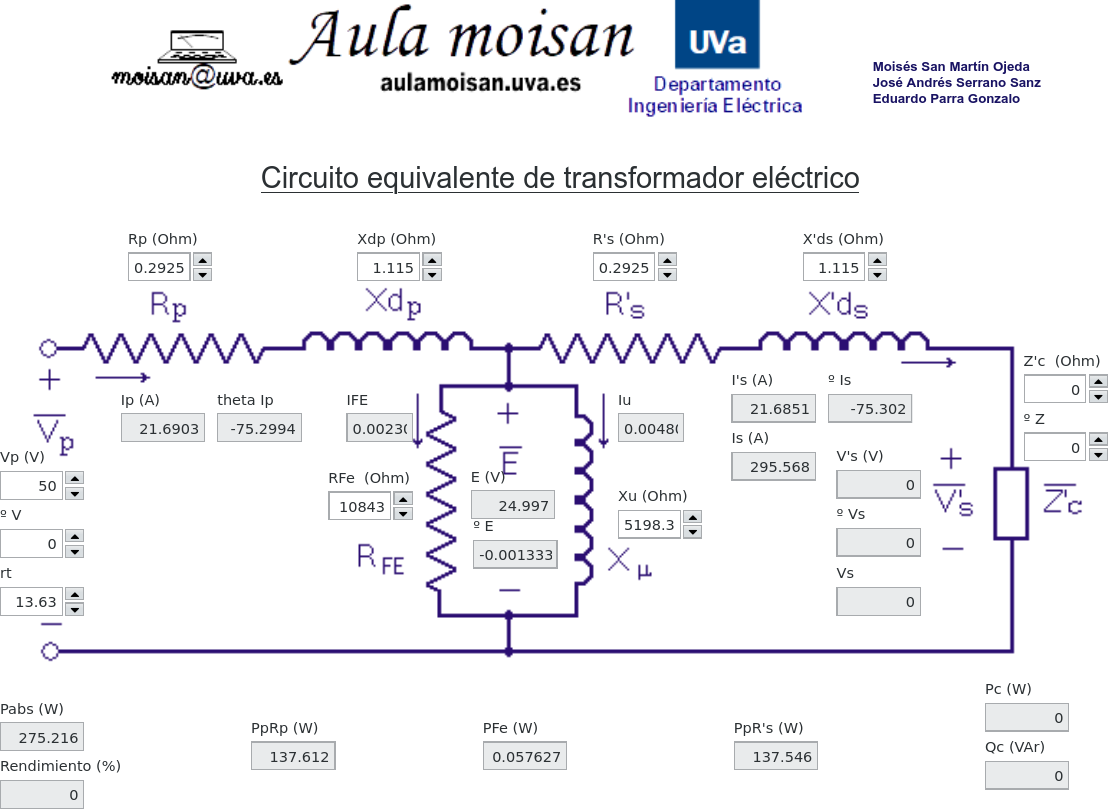
\includegraphics[width=\textwidth]{images/fig_cc_controlado_50V.png}
        \caption{$V_p = \SI{50}{\volt}$.}
        \label{fig.anexo:cc_50V}
    \end{subfigure}
\end{figure}
\begin{figure}[!ht]
    \ContinuedFloat
    \centering
    \begin{subfigure}[t]{0.48\textwidth}
        \centering
        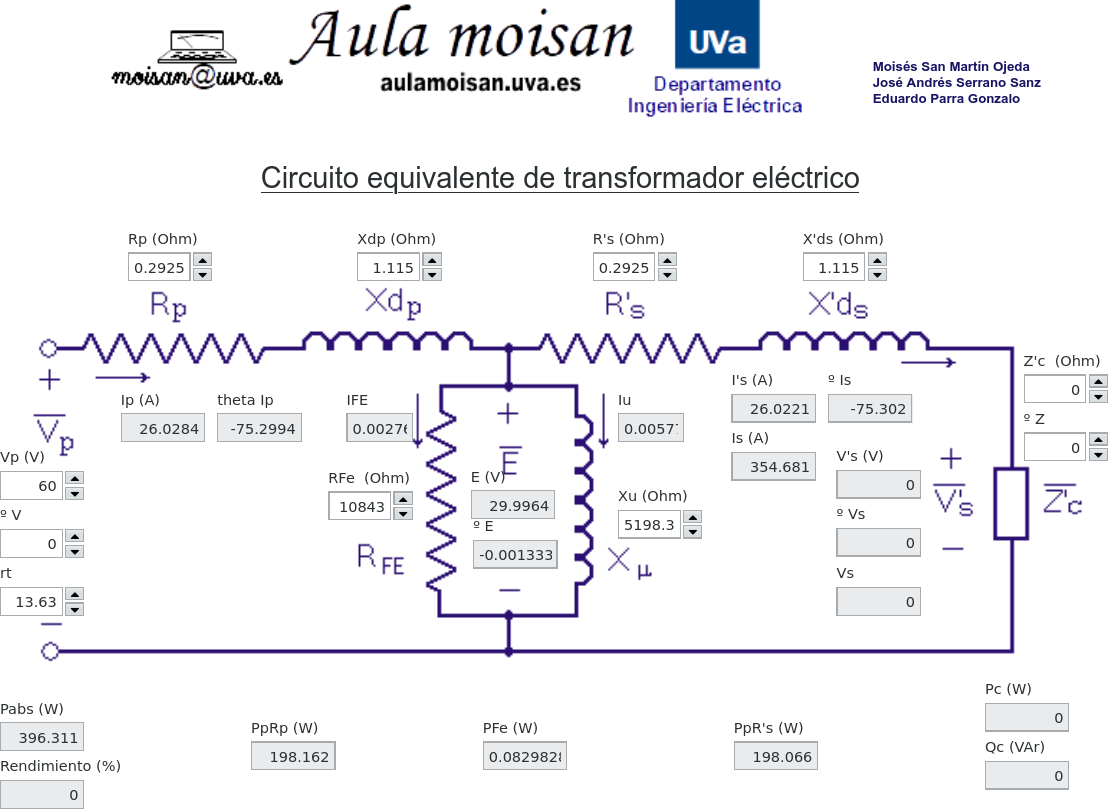
\includegraphics[width=\textwidth]{images/fig_cc_controlado_60V.png}
        \caption{$V_p = \SI{60}{\volt}$.}
        \label{fig.anexo:cc_60V}
    \end{subfigure}
    \hfill
    \begin{subfigure}[t]{0.48\textwidth}
        \centering
        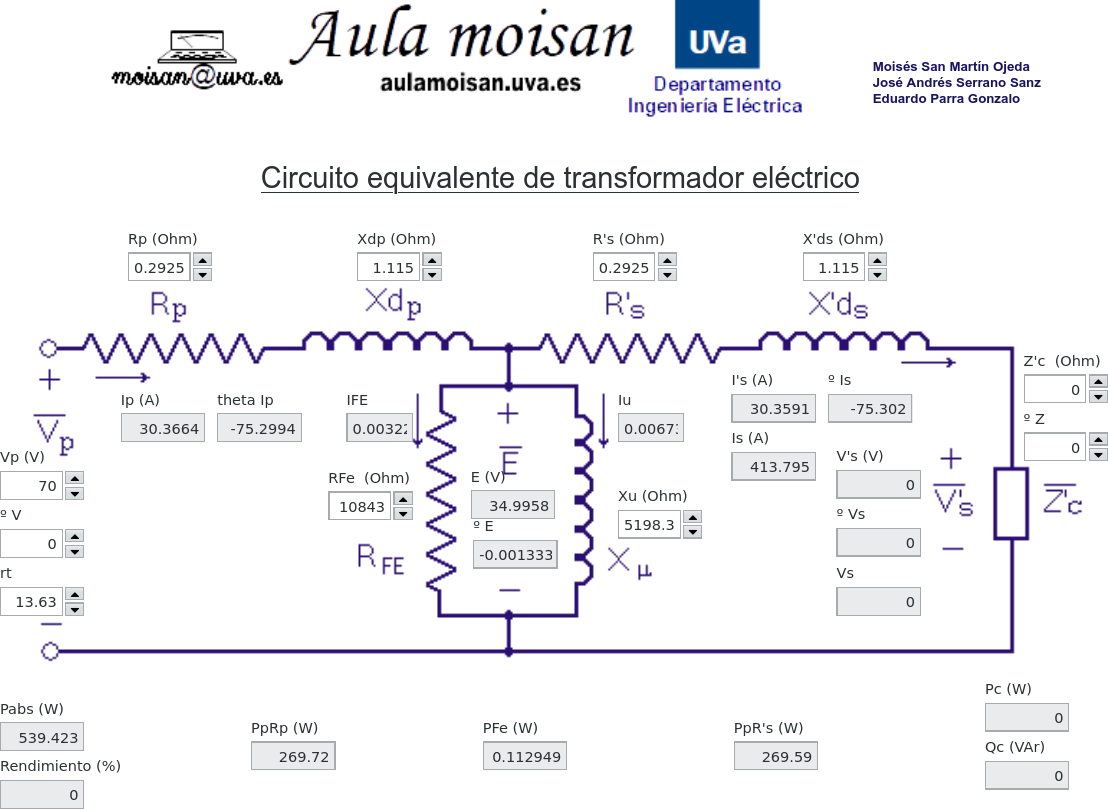
\includegraphics[width=\textwidth]{images/fig_cc_controlado_70V.png}
        \caption{$V_p = \SI{70}{\volt}$.}
        \label{fig.anexo:cc_70V}
    \end{subfigure}
    \vskip\baselineskip
    \begin{subfigure}[t]{0.48\textwidth}
        \centering
        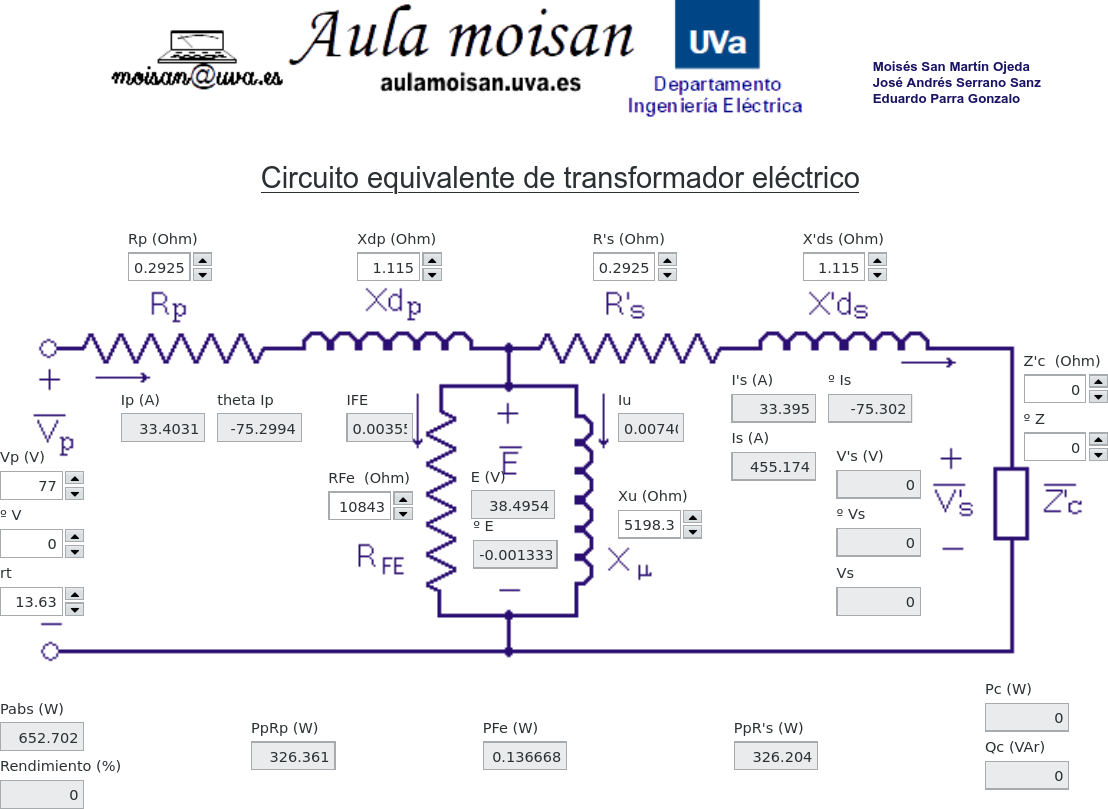
\includegraphics[width=\textwidth]{images/fig_cc_controlado_77V.png}
        \caption{$V_p = \SI{77}{\volt}$ (nominal).}
        \label{fig.anexo:cc_controlado_77V}
    \end{subfigure}
    \caption{Barrido de tensión en el ensayo de cortocircuito controlado.}
    \label{fig.anexo:cc_barrido}
\end{figure}

\begin{figure}[!ht]
    \centering
    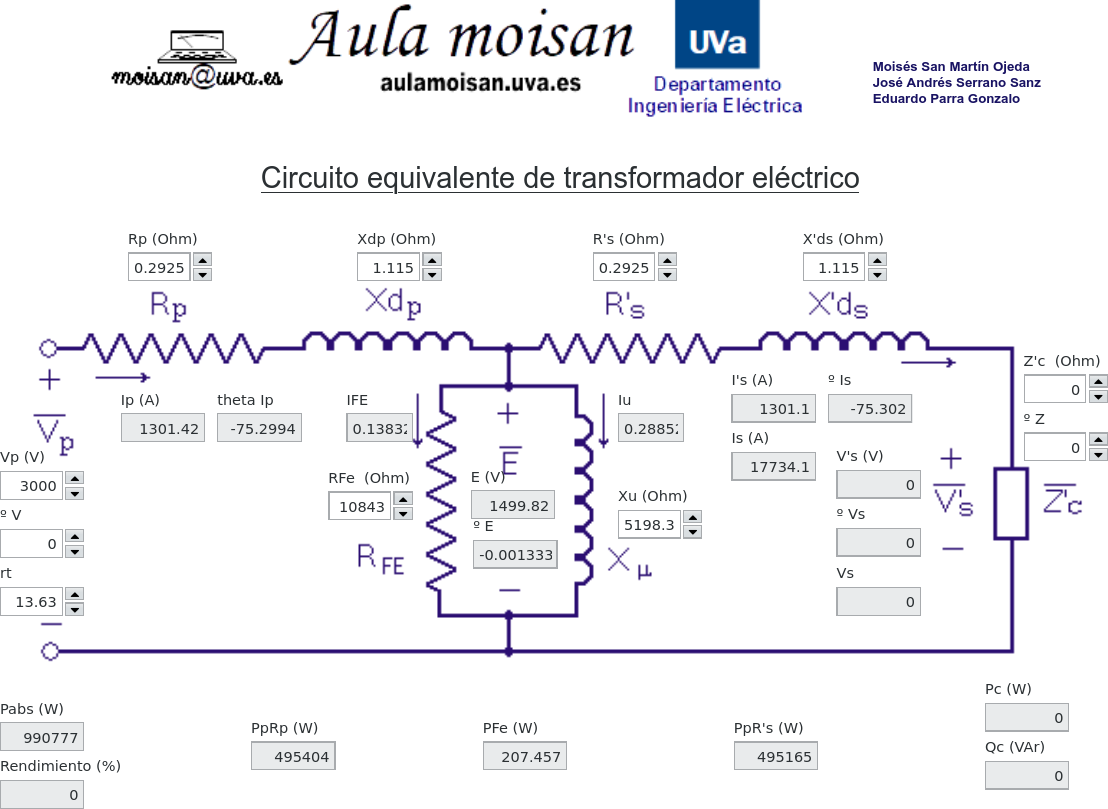
\includegraphics[width=0.7\textwidth]{images/fig_cc_franco.png}
    \caption{Cortocircuito franco ($V_p = \SI{3000}{\volt}, Z'_c = 0$).}
    \label{fig.anexo:cc_franco}
\end{figure}
